%%%%%%%%%%%%%%%%%%%%%%%%%%%%%%%%%%%%%%%%%
% Beamer Presentation
% LaTeX Template
% Version 1.0 (10/11/12)
%
% This template has been downloaded from:
% http://www.LaTeXTemplates.com
%
% License:
% CC BY-NC-SA 3.0 (http://creativecommons.org/licenses/by-nc-sa/3.0/)
%
%%%%%%%%%%%%%%%%%%%%%%%%%%%%%%%%%%%%%%%%%

%----------------------------------------------------------------------------------------
%    PACKAGES AND THEMES
%----------------------------------------------------------------------------------------

%%TO COMPILE AND GENERATE THE INDEX
%pdflatex TRUST_tutorial.tex
%pdflatex TRUST_tutorial.tex

\documentclass[10pt, hyperref={unicode=true,pdfusetitle, bookmarks=true,bookmarksnumbered=false,bookmarksopen=false, breaklinks=false,pdfborder={0 0 1},backref=true,colorlinks=true,linkcolor=darkblue,pageanchor, urlcolor=darkblue}]{beamer}

\mode<presentation> {

% The Beamer class comes with a number of default slide themes
% which change the colors and layouts of slides. Below this is a list
% of all the themes, uncomment each in turn to see what they look like.

%\usetheme{default}
%\usetheme{AnnArbor}
%\usetheme{Antibes}
%\usetheme{Bergen}
%\usetheme{Berkeley}
%\usetheme{Berlin}
%\usetheme{Boadilla}
\usetheme{CambridgeUS}
%\usetheme{Copenhagen}
%\usetheme{Darmstadt}
%\usetheme{Dresden}
%\usetheme{Frankfurt}
%\usetheme{Goettingen}
%\usetheme{Hannover}
%\usetheme{Ilmenau}
%\usetheme{JuanLesPins}
%\usetheme{Luebeck}
%\usetheme{Madrid}
%\usetheme{Malmoe}
%\usetheme{Marburg}
%\usetheme{Montpellier}
%\usetheme{PaloAlto}
%\usetheme{Pittsburgh}
%\usetheme{Rochester}
%\usetheme{Singapore}
%\usetheme{Szeged}
%\usetheme{Warsaw}

% As well as themes, the Beamer class has a number of color themes
% for any slide theme. Uncomment each of these in turn to see how it
% changes the colors of your current slide theme.

%\usecolortheme{albatross} % bleubleu
%\usecolortheme{beaver} % rouge
%\usecolortheme{beetle} % bleu/gris
%\usecolortheme{crane}  % jaune
%\usecolortheme{dolphin} % bleu
%\usecolortheme{dove}  % blanc
%\usecolortheme{fly} % gris
%\usecolortheme{lily} % bleu
%\usecolortheme{orchid} % bleu
%\usecolortheme{rose} % bleu
%\usecolortheme{seagull} % gris
%\usecolortheme{seahorse} % bleu pale
%\usecolortheme{whale} % bleu
%\usecolortheme{wolverine} % jaune/bleu

%\setbeamertemplate{footline} % To remove the footer line in all slides uncomment this line
%\setbeamertemplate{footline}[page number] % To replace the footer line in all slides with a simple slide count uncomment this line

%\setbeamertemplate{navigation symbols}{} % To remove the navigation symbols from the bottom of all slides uncomment this line

}

\usepackage{graphicx} % Allows including images
\definecolor{darkblue}{HTML}{3535B4}
\definecolor{Greeen}{HTML}{439236}
\definecolor{vert}{HTML}{0ab351}
\definecolor{LightSkyBlue}{HTML}{87CFFA}
\usepackage[T1]{fontenc}
\usepackage{alltt}
\usepackage{tikz}

%----------------------------------------------------------------------------------------
%    TITLE PAGE
%----------------------------------------------------------------------------------------
%\title[Short title]{Long title}
\title[TRUST ICoCo Tutorial V1.9.6]{TRUST ICoCo Tutorial V1.9.6}
% The short title appears at the bottom of every slide, the full title is only on the title page

%\author{John Smith} % Your name
\institute[CEA/DES/ISAS/DM2S] % Your institution as it will appear on the bottom of every slide, may be shorthand to save space
{
CEA Saclay \\ % Your institution for the title page
\medskip
\textit{Support team: trust@cea.fr} % Your email address
\medskip
}
\date{\today} % Date, can be changed to a custom date


\begin{document}

%%%%%%%%%%%%%%%%%%%%%%%%%%%%%%%%%%%%%%%%%%%%%%%%%%%%%%%%%%%%%%%%%%%%%%%%
\begin{frame}
\titlepage % Print the title page as the first slide
\end{frame}
%%%%%%%%%%%%%%%%%%%%%%%%%%%%%%%%%%%%%%%%%%%%%%%%%%%%%%%%%%%%%%%%%%%%%%%%

%----------------------------------------------------------------------------------------
%    PRESENTATION SLIDES
%----------------------------------------------------------------------------------------
%%%%%%%%%%%%%%%%%%%%%%%%%%%%%%%%%%%%%%%%%%%%%%%%%%%%%%%%%%%%%%%%%%%%%%%%
\begin{frame}
\tableofcontents [hideallsubsections]
%\begin{columns}[c] 
%\column{.45\textwidth}
%\tableofcontents[sections={1-3},hideallsubsections]
%\column{.5\textwidth} 
%\tableofcontents[sections={4-8},hideallsubsections]
%\end{columns}
\end{frame}
%%%%%%%%%%%%%%%%%%%%%%%%%%%%%%%%%%%%%%%%%%%%%%%%%%%%%%%%%%%%%%%%%%%%%%%%



\section{{\bf{Introduction to code coupling and ICoCo}}}
%%%%%%%%%%%%%%%%%%%%%%%%%%%%%%%%%%%%%%%%%%%%%%%%%%%%%%%%%%%%%%%%%%%%%%%%
%\begin{frame}
%\tableofcontents[currentsection, currentsubsection]
%\end{frame}
%%%%%%%%%%%%%%%%%%%%%%%%%%%%%%%%%%%%%%%%%%%%%%%%%%%%%%%%%%%%%%%%%%%%%%%%
%%%%%%%%%%%%%%%%%%%%%%%%%%%%%%%%%%%%%%%%%%%%%%%%%%%%%%%%%%%%%%%%%%%%%%%%
\begin{frame}
\frametitle{Why code coupling?}
\begin{block}{Code coupling ... what for ?}

\begin{columns}[c] 
\column{.6\textwidth}
\begin{itemize}
\item Traditionnaly \textit{numerical simulation codes} focus on a single physics
    \begin{itemize}
    \item [$\circ$] One code for thermics
    \item [$\circ$] Another code for mechanics,
    \item [$\circ$] Etc...
    \end{itemize}
\item Real life studies require the simulation of different physics
    \begin{itemize}
    \item [$\circ$] E.g. nuclear reactor simulations require a blend of: thermics, neutronics, mechanics...
    \end{itemize}
\item Solution? Code coupling!
    \begin{itemize}
    \item [$\circ$] Have different codes communicating one with another...
    \item [$\circ$] while each code deals with its own area of expertise
    \end{itemize}
\end{itemize}

\column{.4\textwidth} 
\begin{figure}[H]
\begin{centering}
\includegraphics[scale=0.5]{PICTURES/Image1.png}
\par\end{centering}
\end{figure}
\end{columns}

\end{block}
\end{frame}
%%%%%%%%%%%%%%%%%%%%%%%%%%%%%%%%%%%%%%%%%%%%%%%%%%%%%%%%%%%%%%%%%%%%%%%%
%%%%%%%%%%%%%%%%%%%%%%%%%%%%%%%%%%%%%%%%%%%%%%%%%%%%%%%%%%%%%%%%%%%%%%%%
\begin{frame}
\frametitle{Code coupling}
\begin{block}{First approach}

\begin{itemize}
\item An entity driving the complete computation is needed: the \textbf{\textcolor{LightSkyBlue}{supervisor}}
    \begin{itemize}
    \item [$\circ$] Initializes code A and code B
    \item [$\circ$] Loop through code A and code B
    \item [$\circ$] Centralize exchanges and conversions between A and B
\end{itemize}
Supervisor is usually written from scratch as a C++ program, Python script, $\cdots$

\item In a dummy approach : supervisor needs to know \textit{both} A and B API. \\
It becomes cumbersome if :
    \begin{itemize}
    \item [$\circ$] more than 2 codes to couple ...
    \item [$\circ$] single supervisor is meant to run with different pairs of codes (code C, D, E ...)
    \end{itemize}
\end{itemize}

\begin{figure}[h!]
\begin{center}
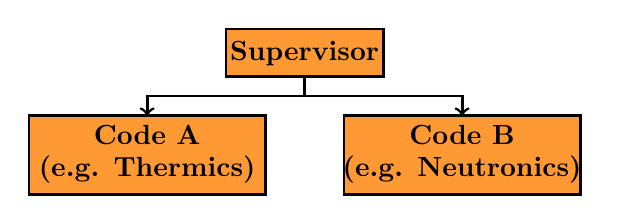
\begin{tikzpicture}[scale=1, line width=1pt]
% box Supervisor
\coordinate (A) at (2.5,1.5) ;
\coordinate (B) at (4.5,1.5) ;
\coordinate (C) at (4.5,2.1) ;
\coordinate (D) at (2.5,2.1) ;
\draw[black,fill=orange!80] (A) -- (B) -- (C) -- (D) -- cycle ;
\draw (3.5,1.5) node[above]{\textbf{Supervisor}} ;
%% box Code A
\begin{scope}
\coordinate (A1) at (0,0) ;
\coordinate (B1) at (3,0) ;
\coordinate (C1) at (3,1) ;
\coordinate (D1) at (0,1) ;
\draw[black,fill=orange!80] (A1) -- (B1) -- (C1) -- (D1) -- cycle ;
\draw (1.5,0.5) node[above]{\textbf{Code A}} ;
\draw (1.5,0.) node[above]{\textbf{(e.g. Thermics)}} ;
\end{scope}
%% box Code B
\begin{scope}
\coordinate (A2) at (4,0) ;
\coordinate (B2) at (7,0) ;
\coordinate (C2) at (7,1) ;
\coordinate (D2) at (4,1) ;
\draw[black,fill=orange!80] (A2) -- (B2) -- (C2) -- (D2) -- cycle ;
\draw (5.5,0.5) node[above]{\textbf{Code B}} ;
\draw (5.5,0.) node[above]{\textbf{(e.g. Neutronics)}} ;
\end{scope}
\draw [->] (3.5,1.5) -- (3.5,1.25) -- (1.5,1.25) -- (1.5,1);
\draw [->] (3.5,1.5) -- (3.5,1.25) -- (5.5,1.25) -- (5.5,1);
\end{tikzpicture}
\end{center}
\end{figure}

\end{block}
\end{frame}
%%%%%%%%%%%%%%%%%%%%%%%%%%%%%%%%%%%%%%%%%%%%%%%%%%%%%%%%%%%%%%%%%%%%%%%%
%%%%%%%%%%%%%%%%%%%%%%%%%%%%%%%%%%%%%%%%%%%%%%%%%%%%%%%%%%%%%%%%%%%%%%%%
\begin{frame}
\frametitle{Code coupling}
\begin{block}{Better: common interface!}


\underline{\textbf{Idea}}: define a unique \textit{interface} to which each code must comply
    \begin{itemize}
    \item [$\circ$] Only an \textit{interface}, i.e. a contract (=an API) that each code fulfills
    \item [$\circ$] \textit{Implementation} (=plugging wires) of this interface is tightly linked to the details of the code...
    \end{itemize}
Advantages:
    \begin{itemize}
    \item [$\circ$] All codes implementing the (unique) interface can be passed to the supervisor (almost) without modifying it! \textbf{\textcolor{LightSkyBlue}{Versatility}}
    \end{itemize}
Constraints:
    \begin{itemize}
    \item [$\circ$] Need to implement the interface for each code to be coupled
    \end{itemize}

\begin{figure}[h!]
\begin{center}
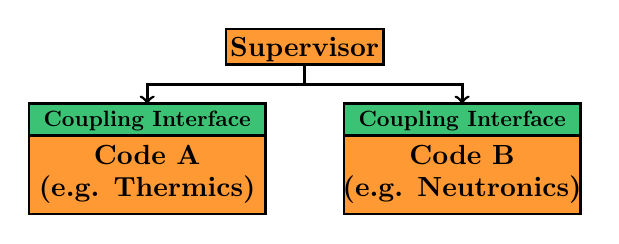
\begin{tikzpicture}[scale=1, line width=1pt]
% box Supervisor
\coordinate (A) at (2.5,1.5) ;
\coordinate (B) at (4.5,1.5) ;
\coordinate (C) at (4.5,1.95) ;
\coordinate (D) at (2.5,1.95) ;
\draw[black,fill=orange!80] (A) -- (B) -- (C) -- (D) -- cycle ;
\draw (3.5,1.4) node[above]{\textbf{Supervisor}} ;
%% box Code A
\begin{scope}
\coordinate (A1) at (0,-0.4) ;
\coordinate (B1) at (3,-0.4) ;
\coordinate (C1) at (3,0.6) ;
\coordinate (D1) at (0,0.6) ;
\coordinate (E1) at (0,1) ;
\coordinate (F1) at (3,1) ;
\draw[black,fill=orange!80] (A1) -- (B1) -- (C1) -- (D1) -- cycle ;
\draw[black,fill=vert!80] (C1) -- (D1) -- (E1) -- (F1)-- cycle ;
\draw (1.5,0.55) node[above,scale=0.8]{\textbf{Coupling Interface}} ;
\draw (1.5,0.1) node[above]{\textbf{Code A}} ;
\draw (1.5,-0.4) node[above]{\textbf{(e.g. Thermics)}} ;
\end{scope}
%% box Code B
\begin{scope}
\coordinate (A2) at (4,-0.4) ;
\coordinate (B2) at (7,-0.4) ;
\coordinate (C2) at (7,0.6) ;
\coordinate (D2) at (4,0.6) ;
\coordinate (E2) at (4,1) ;
\coordinate (F2) at (7,1) ;
\draw[black,fill=orange!80] (A2) -- (B2) -- (C2) -- (D2) -- cycle ;
\draw[black,fill=vert!80] (C2) -- (D2) -- (E2) -- (F2)-- cycle ;
\draw (5.5,0.55) node[above,scale=0.8]{\textbf{Coupling Interface}} ;
\draw (5.5,0.1) node[above]{\textbf{Code B}} ;
\draw (5.5,-0.4) node[above]{\textbf{(e.g. Neutronics)}} ;
\end{scope}
\draw [->] (3.5,1.5) -- (3.5,1.25) -- (1.5,1.25) -- (1.5,1);
\draw [->] (3.5,1.5) -- (3.5,1.25) -- (5.5,1.25) -- (5.5,1);
\end{tikzpicture}
\end{center}
\end{figure}

\end{block}
\end{frame}
%%%%%%%%%%%%%%%%%%%%%%%%%%%%%%%%%%%%%%%%%%%%%%%%%%%%%%%%%%%%%%%%%%%%%%%%
%%%%%%%%%%%%%%%%%%%%%%%%%%%%%%%%%%%%%%%%%%%%%%%%%%%%%%%%%%%%%%%%%%%%%%%%
\begin{frame}
\frametitle{ICoCo, \textbf{I}nterface for \textbf{Co}de \textbf{Co}upling}
\begin{block}{}

ICoCo is such a coupling interface:
\begin{itemize}
\item Stands for \textbf{I}nterface for \textbf{Co}de \textbf{Co}upling
\item Written in C++ (and in swig since TRUST-1.8.3 to be used through Python)
\vspace{0.2cm}
\item Initially designed for simulation codes exhibiting \textbf{\textcolor{LightSkyBlue}{iterative time loops}} 
\vspace{0.2cm}
\item Presents a set of standard methods whose signature is fixed, with no default implementation:
    \begin{itemize}
    \item [$\circ$] initializeTimeStep()
    \item [$\circ$] validateTimeStep()
    \item [$\circ$] abortTimeStep()
    \item [$\circ$] ...
    \end{itemize}
\item Uses the notion of field for data exchange between codes
    \begin{itemize}
    \item [$\circ$] A field is a set of values supported by a mesh
    \item [$\circ$] A possible implementation: \textbf{MEDCouplingFieldDouble}, from SALOME's MEDCoupling library
    \end{itemize}
\end{itemize}

\end{block}
\end{frame}
%%%%%%%%%%%%%%%%%%%%%%%%%%%%%%%%%%%%%%%%%%%%%%%%%%%%%%%%%%%%%%%%%%%%%%%%
%%%%%%%%%%%%%%%%%%%%%%%%%%%%%%%%%%%%%%%%%%%%%%%%%%%%%%%%%%%%%%%%%%%%%%%%
\begin{frame}
\frametitle{Further reading}
\begin{block}{Meaningful documentation}

\begin{itemize}
\item ICOCO presentation in TRUST documentation: \\ \textbf{"An Interface for Code Coupling ICoCo v1.2"} \\
    \hspace{0.5cm}\texttt{load TRUST environnement} \\
    \hspace{0.5cm}\texttt{\$ evince \$TRUST\_ROOT/doc/Kernel/ICoCo\_V1.2.pdf \&}
    \vspace{0.2cm}

    \item Ask the "APIProblem.pdf" note to trust@cea.fr
\end{itemize}

\end{block}
\end{frame}
%%%%%%%%%%%%%%%%%%%%%%%%%%%%%%%%%%%%%%%%%%%%%%%%%%%%%%%%%%%%%%%%%%%%%%%%



\section{{\bf{TRUST and ICoCo initialization}}}
%%%%%%%%%%%%%%%%%%%%%%%%%%%%%%%%%%%%%%%%%%%%%%%%%%%%%%%%%%%%%%%%%%%%%%%%
\begin{frame}
\tableofcontents[currentsection, currentsubsection]
\end{frame}

%%%%%%%%%%%%%%%%%%%%%%%%%%%%%%%%%%%%%%%%%%%%%%%%%%%%%%%%%%%%%%%%%%%%%%%%
%%%%%%%%%%%%%%%%%%%%%%%%%%%%%%%%%%%%%%%%%%%%%%%%%%%%%%%%%%%%%%%%%%%%%%%%
%%%%%%%%%%%%%%%%%%%%%%%%%%%%%%%%%%%%%%%%%%%%%%%%%%%%%%%%%%%%%%%%%%%%%%%%
%%%%%%%%%%%%%%%%%%%%%%%%%%%%%%%%%%%%%%%%%%%%%%%%%%%%%%%%%%%%%%%%%%%%%%%%
\begin{frame}
\subsection{Initialization of TRUST environment}

\frametitle{Initialization of TRUST environment}
\begin{block}{}

\begin{itemize}
\item Before starting this Tutorial, \\
 it is highly recommended to know some TRUST commands and hints.\vspace{0.2cm}
 \item Source the TRUST environment:\\
\begin{itemize}
\item On CEA Saclay PCs, TRUST versions are available with:\\
\textbf{source /home/triou/env\_TRUST\_1.9.5.sh}
\vspace{0.2cm}
\item On your own computer, download and install the latest version of TRUST in your local folder \$MyPathToTRUSTversion (unless this was already performed), then write on the terminal:\\
%\vspace{0.2cm}
\textbf{source  \$MyPathToTRUSTversion/env\_TRUST.sh}
\vspace{0.2cm}
\end{itemize}

\item To check if the configuration is well and to locate sources:\\
\texttt{\$ echo \$TRUST\_ROOT}
%\vspace{0.2cm}
\end{itemize}
\end{block}
\end{frame}
%%%%%%%%%%%%%%%%%%%%%%%%%%%%%%%%%%%%%%%%%%%%%%%%%%%%%%%%%%%%%%%%%%%%%%%%
%%%%%%%%%%%%%%%%%%%%%%%%%%%%%%%%%%%%%%%%%%%%%%%%%%%%%%%%%%%%%%%%%%%%%%%%

\begin{frame}
\subsection{Initialization of ICoCo environment}
\frametitle{Initialization of ICoCo environment}
\begin{block}{}

\begin{itemize}

\item Source the ICoCo environment:\\
\hspace{-0.5cm}\texttt{\$ source \$TRUST\_ROOT/Outils/ICoCo/ICoCo\_src/full\_env\_MEDICoCo.sh}

\item check if ICoCo is compiled:\\
\texttt{\$ ls \$exec} 

\item If you obtain "ls: cannot access **/Outils/ICoCo/ICoCo\_src/ICoCo\_opt: No such file or directory", then compile ICoCo\_src:\\
\texttt{\$ cd \$TRUST\_ROOT/Outils/ICoCo/ICoCo\_src}\\
\texttt{\$ baltik\_build\_configure -execute}\\
\texttt{\$ make optim debug }\\
\texttt{\$ source full\_env\_MEDICoCo.sh}

\item If you do not have rights to compile ICoCo (Typically if TRUST install is made by someone else): \\
\texttt{\$ mkdir -p ICoCo}\\
\texttt{\$ cp -r \$TRUST\_ROOT/Outils/ICoCo/ICoCo\_src ICoCo/ICoCo\_src}\\
\texttt{\$ cd ICoCo/ICoCo\_src}\\
\texttt{\$ baltik\_build\_configure -execute ; make optim debug }\\
\texttt{\$ source full\_env\_MEDICoCo.sh}

\end{itemize}

\end{block}
\end{frame}
%%%%%%%%%%%%%%%%%%%%%%%%%%%%%%%%%%%%%%%%%%%%%%%%%%%%%%%%%%%%%%%%%%%%%%%%
%%%%%%%%%%%%%%%%%%%%%%%%%%%%%%%%%%%%%%%%%%%%%%%%%%%%%%%%%%%%%%%%%%%%%%%%


\section{{\bf{Basic test case}}}
%%%%%%%%%%%%%%%%%%%%%%%%%%%%%%%%%%%%%%%%%%%%%%%%%%%%%%%%%%%%%%%%%%%%%%%%
\begin{frame}
\tableofcontents[currentsection, currentsubsection]
\end{frame}
%%%%%%%%%%%%%%%%%%%%%%%%%%%%%%%%%%%%%%%%%%%%%%%%%%%%%%%%%%%%%%%%%%%%%%%%

%%%%%%%%%%%%%%%%%%%%%%%%%%%%%%%%%%%%%%%%%%%%%%%%%%%%%%%%%%%%%%%%%%%%%%%%
\begin{frame}
\frametitle{Goal of this first exercise}
\begin{block}{}
The idea here is to:

\begin{enumerate}
\item  Create a reference test case 
\begin{itemize}
\item To be launched with TRUST executable.
\end{itemize}\vspace{0.1cm}
\item Update the test case in order to:
\begin{itemize}
\item Launch it sequentially with ICoCo without information exchange.
\item  Ensure that obtained results are identical to those obtained in step 1.
\end{itemize}\vspace{0.1cm}
\item Realize your first information exchange between the supervisor and datafile
\begin{itemize}
\item Impose a boundary condition from the supervisor and launch the calculation sequentially with ICoCo
\item Compare the results with those obtained with TRUST executable.
\end{itemize}\vspace{0.1cm}
\item Make the test case running with ICoCo in parallel:
\begin{itemize}
\item Launch the computation with ICoCo on 2 processes \item Compare obtained results with those with TRUST executable.
\end{itemize}
\end{enumerate}

\end{block}
\end{frame}
%%%%%%%%%%%%%%%%%%%%%%%%%%%%%%%%%%%%%%%%%%%%%%%%%%%%%%%%%%%%%%%%%%%%%%%%


\subsection{{\bf{TRUST: test case creation}}}
%%%%%%%%%%%%%%%%%%%%%%%%%%%%%%%%%%%%%%%%%%%%%%%%%%%%%%%%%%%%%%%%%%%%%%%%
\begin{frame}
\tableofcontents[currentsection, currentsubsection]
\end{frame}
%%%%%%%%%%%%%%%%%%%%%%%%%%%%%%%%%%%%%%%%%%%%%%%%%%%%%%%%%%%%%%%%%%%%%%%%
%%%%%%%%%%%%%%%%%%%%%%%%%%%%%%%%%%%%%%%%%%%%%%%%%%%%%%%%%%%%%%%%%%%%%%%%
\begin{frame}
\frametitle{TRUST: test case creation}
\begin{block}{}
We will copy a reference test case from TRUST tests database that we launch with TRUST. 

\begin{itemize}
\item Copy Vahl\_Davis\_hexa test case in your repository:\\
\texttt{\$ mkdir ICoCo\_exercises}\\
\texttt{\$ cd ICoCo\_exercises}\\
\texttt{\$ trust -copy Vahl\_Davis\_hexa}
\item Rename the folder to distinguish your tests:\\
\texttt{\$ mv Vahl\_Davis\_hexa Vahl\_Davis\_hexa\_trust}\\
\texttt{\$ cd Vahl\_Davis\_hexa\_trust}
\item Rename the datafile to be consistent with the folder's name:\\
\texttt{\$ mv Vahl\_Davis\_hexa.data Vahl\_Davis\_hexa\_trust.data}\\
\item Launch calculation:\\
\texttt{\$ trust Vahl\_Davis\_hexa\_trust}\\
\item You obtained a Vahl\_Davis\_hexa\_trust.lml file. We will need it in the following part.
\end{itemize}

\end{block}
\end{frame}
%%%%%%%%%%%%%%%%%%%%%%%%%%%%%%%%%%%%%%%%%%%%%%%%%%%%%%%%%%%%%%%%%%%%%%%%
%%%%%%%%%%%%%%%%%%%%%%%%%%%%%%%%%%%%%%%%%%%%%%%%%%%%%%%%%%%%%%%%%%%%%%%%
\subsection{{\bf{ICoCo: without exchange}}}
\begin{frame}
\frametitle{ICoCo: without exchange}

\begin{block}{Adjusting the datafile}
\begin{itemize}
\item Now let's do the same thing with ICoCo:\\
\texttt{\$ cd ..}\\
\item You are now in the folder "ICoCo\_exercises", create a new directory in order to launch your test case with ICoCo:\\
\texttt{\$ trust -copy Vahl\_Davis\_hexa}\\
\texttt{\$ mv Vahl\_Davis\_hexa Vahl\_Davis\_hexa\_ICoCo}\\
\item Rename the datafile to be consistent with the folder's name:\\
\texttt{\$ cd Vahl\_Davis\_hexa\_ICoCo}\\
\texttt{\$ mv Vahl\_Davis\_hexa.data Vahl\_Davis\_hexa\_ICoCo.data}\\
\item Edit the datafile and add to it ICoCo instructions:
    \begin{itemize}
    \item [$\circ$] \textit{Add} the following line after "\textit{dimension}" definition:\\
    \texttt{Nom ICoCoProblemName Lire ICoCoProblemName pb}
    \item [$\circ$] \textit{Comment} the "\textit{solve pb}" instruction at the end of the datafile.
    \end{itemize}
\end{itemize}
\end{block}

\end{frame}
%%%%%%%%%%%%%%%%%%%%%%%%%%%%%%%%%%%%%%%%%%%%%%%%%%%%%%%%%%%%%%%%%%%%%%%%
%%%%%%%%%%%%%%%%%%%%%%%%%%%%%%%%%%%%%%%%%%%%%%%%%%%%%%%%%%%%%%%%%%%%%%%%
\begin{frame}
\frametitle{ICoCo: without exchange}

\begin{block}{Creation of the main.cpp file}
\begin{itemize}
%\item Create a parallel datafile:\\
%\texttt{\$ trust -partition Vahl\_Davis\_hexa}\\
\item Create the main.cpp which will launch the calculation:\\
\texttt{\$ file="main\_Vahl\_Davis\_hexa\_ICoCo.cpp"} \\
\texttt{\$ cp \$TRUST\_ROOT/doc/TRUST/exercices/ICoCo/\$file main.cpp}\\
\item Open main.cpp file and see the main method which creates the objects and launches computation.
\item You can use ICoCo with 1 or more processors, but in this part we use only one processor to solve the problem.
%\item You can also see where the datafile and in/output files are set.
%\item Here we only run the calculation with the "while" loop.
\end{itemize}
\end{block}

\begin{block}{Creation of the makefile}
\begin{itemize}
\item Create a makefile for your calculation:\\
\texttt{\$ cp \$project\_directory/share/bin/create\_Makefile .} \\
\texttt{\$ sh create\_Makefile}
\item Compile it:\\
\texttt{\$ make}
\item This creates an executable "couplage" and a datafile "couplage.data".
\end{itemize}

\end{block}
\end{frame}
%%%%%%%%%%%%%%%%%%%%%%%%%%%%%%%%%%%%%%%%%%%%%%%%%%%%%%%%%%%%%%%%%%%%%%%%
%%%%%%%%%%%%%%%%%%%%%%%%%%%%%%%%%%%%%%%%%%%%%%%%%%%%%%%%%%%%%%%%%%%%%%%%
\begin{frame}
\frametitle{ICoCo: without exchange}

\begin{block}{Launch calculation}
\begin{itemize}
\item Execute it:\\
\texttt{\$./couplage}
%\texttt{\$ mpirun -np 2 ./couplage}
\item You should obtain the same results as with TRUST executable. Compare TRUST and ICoCo results with:\\
\texttt{\$ compare\_lata Vahl\_Davis\_hexa\_ICoCo.lml ../Vahl\_Davis\_hexa\_trust/Vahl\_Davis\_hexa\_trust.lml}
\item Both lml files are identical!
\end{itemize}

\end{block}
\end{frame}
%%%%%%%%%%%%%%%%%%%%%%%%%%%%%%%%%%%%%%%%%%%%%%%%%%%%%%%%%%%%%%%%%%%%%%%%
%%%%%%%%%%%%%%%%%%%%%%%%%%%%%%%%%%%%%%%%%%%%%%%%%%%%%%%%%%%%%%%%%%%%%%%%



\subsection{{\bf{ICoCo: first input}}}
%%%%%%%%%%%%%%%%%%%%%%%%%%%%%%%%%%%%%%%%%%%%%%%%%%%%%%%%%%%%%%%%%%%%%%%%
\begin{frame}
\tableofcontents[currentsection, currentsubsection]
\end{frame}
%%%%%%%%%%%%%%%%%%%%%%%%%%%%%%%%%%%%%%%%%%%%%%%%%%%%%%%%%%%%%%%%%%%%%%%%
%%%%%%%%%%%%%%%%%%%%%%%%%%%%%%%%%%%%%%%%%%%%%%%%%%%%%%%%%%%%%%%%%%%%%%%%
\begin{frame}
\frametitle{ICoCo: first input}
\begin{block}{Adjusting the main.cpp file}

\begin{itemize}
\item Copy the following test case in your repository:\\
\texttt{\$ cd ..}\\
\texttt{\$ cp -r Vahl\_Davis\_hexa\_ICoCo Vahl\_Davis\_hexa\_ICoCo\_exchange}\\
\texttt{\$ cd Vahl\_Davis\_hexa\_ICoCo\_exchange}\\
\item Clean the repository and rename the datafile:\\
\texttt{\$ trust -clean}\\
\texttt{\$ mv Vahl\_Davis\_hexa\_ICoCo.data Vahl\_Davis\_hexa\_ICoCo\_exchange.data }\\
%\item We want to create an input of temperature with the first domain. So you have to create a new domain:\\
%\textit{  set<int> dom2\_ids;}
%\item And create objects which will made the input, add the following lines after the "synchronize\_bool(stop,sync\_or);" line:\\
%\textit{  TrioDEC dec\_temperature(dom2\_ids, dom1\_ids);}\\
%\textit{  TrioField Temperature\_field;}
\item We will add a block in the main.cpp file to exchange values.
\item Copy the following file in your folder:\\
\texttt{\$ file="main\_Vahl\_Davis\_hexa\_ICoCo\_exchange.cpp"}\\ 
\texttt{\$ cp \$TRUST\_ROOT/doc/TRUST/exercices/ICoCo/\$file main.cpp}
\end{itemize}

\end{block}
\end{frame}
%%%%%%%%%%%%%%%%%%%%%%%%%%%%%%%%%%%%%%%%%%%%%%%%%%%%%%%%%%%%%%%%%%%%%%%%
%%%%%%%%%%%%%%%%%%%%%%%%%%%%%%%%%%%%%%%%%%%%%%%%%%%%%%%%%%%%%%%%%%%%%%%%
\begin{frame}
\frametitle{ICoCo: first input}
\begin{block}{Adjusting the datafile}

\begin{itemize}
\item Then modify the datafile Vahl\_Davis\_hexa\_ICoCo\_exchange.data to make the input:
    \begin{itemize}
    \item [$\circ$] Change the line:\\
    "Gauche Paroi\_temperature\_imposee Champ\_Front\_Uniforme 1 10."\\
     to \\
    "Gauche Paroi\_temperature\_imposee ch\_front\_input \{ nb\_comp 1 nom TEMPERATURE\_IN\_DOM probleme pb \}"
    \item [$\circ$] You can see that the field "TEMPERATURE\_IN\_DOM" is the one employed in the main.cpp file.
%    \item [$\circ$] don't forget to update the parallel datafile:\\
%    \texttt{\$ trust -partition Vahl\_Davis\_hexa}
    \end{itemize}
\end{itemize}

\end{block}
\end{frame}
%%%%%%%%%%%%%%%%%%%%%%%%%%%%%%%%%%%%%%%%%%%%%%%%%%%%%%%%%%%%%%%%%%%%%%%%
%%%%%%%%%%%%%%%%%%%%%%%%%%%%%%%%%%%%%%%%%%%%%%%%%%%%%%%%%%%%%%%%%%%%%%%%
\begin{frame}
\frametitle{ICoCo: first input}
\begin{block}{Launch calculation}

\begin{itemize}
\item Now we can compile and launch the calculation:\\
\texttt{\$ make}\\
\texttt{\$ ./couplage}
\item You may obtain the same results as with TRUST executable.
\item Compare it:\\
\texttt{\$ compare\_lata Vahl\_Davis\_hexa\_ICoCo\_exchange.lml ../Vahl\_Davis\_hexa\_trust/Vahl\_Davis\_hexa\_trust.lml}
\item The files are the same! \textbf{(but not for the first time step!!!!!)}
\end{itemize}

\end{block}
\end{frame}
%%%%%%%%%%%%%%%%%%%%%%%%%%%%%%%%%%%%%%%%%%%%%%%%%%%%%%%%%%%%%%%%%%%%%%%%
%%%%%%%%%%%%%%%%%%%%%%%%%%%%%%%%%%%%%%%%%%%%%%%%%%%%%%%%%%%%%%%%%%%%%%%%



\subsection{{\bf{ICoCo: on 2 processes}}}
%%%%%%%%%%%%%%%%%%%%%%%%%%%%%%%%%%%%%%%%%%%%%%%%%%%%%%%%%%%%%%%%%%%%%%%%
\begin{frame}
\tableofcontents[currentsection, currentsubsection]
\end{frame}
%%%%%%%%%%%%%%%%%%%%%%%%%%%%%%%%%%%%%%%%%%%%%%%%%%%%%%%%%%%%%%%%%%%%%%%%
%%%%%%%%%%%%%%%%%%%%%%%%%%%%%%%%%%%%%%%%%%%%%%%%%%%%%%%%%%%%%%%%%%%%%%%%
\begin{frame}
\frametitle{ICoCo: on 2 processes}
\begin{block}{Adjusting the main.cpp file}

\begin{itemize}
\item Copy the following test case in your repository:\\
\texttt{\$ cd ..}\\
\texttt{\$ cp -r Vahl\_Davis\_hexa\_ICoCo\_exchange Vahl\_Davis\_hexa\_ICoCo\_para}\\
\texttt{\$ cd Vahl\_Davis\_hexa\_ICoCo\_para}\\
\item Clean the repository and rename the datafile:\\
\texttt{\$ make clean}\\
\texttt{\$ rm main.cpp Vahl\_Davis\_hexa\_ICoCo\_exchange.lml}\\
\texttt{\$ mv Vahl\_Davis\_hexa\_ICoCo\_exchange.data Vahl\_Davis\_hexa\_ICoCo\_para.data }
\item Partition the domaine and create a parallel datafile: \\
\texttt{\$ trust -partition Vahl\_Davis\_hexa\_ICoCo\_para}\\

\item Copy the following file in your folder:\\
\texttt{\$ file="main\_Vahl\_Davis\_hexa\_ICoCo\_para.cpp"}\\
\texttt{\$ cp \$TRUST\_ROOT/doc/TRUST/exercices/ICoCo/\$file main.cpp}\\
\end{itemize}

\end{block}
\end{frame}
%%%%%%%%%%%%%%%%%%%%%%%%%%%%%%%%%%%%%%%%%%%%%%%%%%%%%%%%%%%%%%%%%%%%%%%%
%%%%%%%%%%%%%%%%%%%%%%%%%%%%%%%%%%%%%%%%%%%%%%%%%%%%%%%%%%%%%%%%%%%%%%%%
\begin{frame}
\frametitle{ICoCo: on 2 processes}
\begin{block}{Adjusting the main.cpp file}

\begin{itemize}
\item Open the main.cpp file and search for the MPI command lines.
\item Open this file and look where:
    \begin{itemize}
    \item [$\circ$] the processors are added: search for "dom\_ids"
    \item [$\circ$] the names of the datafiles: search for "data\_file"
    \end{itemize}

\item Create the makefile and coompile your new file:\\
\texttt{\$ sh create\_Makefile}\\
\texttt{\$ make}\\
\item To run parallel, you have to use the following mpirun command:\\
\texttt{\$ mpirun -np 2 ./couplage}\\

\item Compare your results with the sequential ones:\\
\texttt{\$ compare\_lata PAR\_Vahl\_Davis\_hexa\_ICoCo\_para.lml ../Vahl\_Davis\_hexa\_exchange/Vahl\_Davis\_hexa\_exchage.lml}\\
\item Sequential and parallel computation yield the same results!!
\end{itemize}

\end{block}
\end{frame}
%%%%%%%%%%%%%%%%%%%%%%%%%%%%%%%%%%%%%%%%%%%%%%%%%%%%%%%%%%%%%%%%%%%%%%%%



\section{{\bf{Coupled problem with ICoCo}}}
%%%%%%%%%%%%%%%%%%%%%%%%%%%%%%%%%%%%%%%%%%%%%%%%%%%%%%%%%%%%%%%%%%%%%%%%
\begin{frame}
\frametitle{Goal of this second exercise}
\begin{block}{}
The idea here is to:

\begin{enumerate}
\item  Create a reference test case treating a coupled problem 
\begin{itemize}
\item To be launched with TRUST executable in sequential and parallel.
\end{itemize}\vspace{0.1cm}
\item Create two datafiles, each one for a problem:
\begin{itemize} 
\item Launch it with TRUST first to ensure that datafiles do not contain errors
\item Launch it with ICoCo without any information exchange after updating datafiles.
\end{itemize}\vspace{0.1cm}
\item Realize a one way coupling with ICoCo:
\begin{itemize}
\item One way coupling means that one problem runs alone while some inputs of the second problem are provided by the first one 
\item Launch the calculation sequentially with ICoCo
\item Compare the results with those obtained with TRUST executable.
\end{itemize}\vspace{0.1cm}
\item Realize a two-way coupling with ICoCo:
\begin{itemize}
\item Two-way means that each problem will have inputs provided by the other one.
\item Launch the computation with ICoCo.
\end{itemize}
\end{enumerate}

\end{block}
\end{frame}
%%%%%%%%%%%%%%%%%%%%%%%%%%%%%%%%%%%%%%%%%%%%%%%%%%%%%%%%%%%%%%%%%%%%%%%%


\subsection{{\bf{TRUST: test case creation}}}
%%%%%%%%%%%%%%%%%%%%%%%%%%%%%%%%%%%%%%%%%%%%%%%%%%%%%%%%%%%%%%%%%%%%%%%%
\begin{frame}
\tableofcontents[currentsection, currentsubsection]
\end{frame}
%%%%%%%%%%%%%%%%%%%%%%%%%%%%%%%%%%%%%%%%%%%%%%%%%%%%%%%%%%%%%%%%%%%%%%%%
%%%%%%%%%%%%%%%%%%%%%%%%%%%%%%%%%%%%%%%%%%%%%%%%%%%%%%%%%%%%%%%%%%%%%%%%
\begin{frame}
\frametitle{First with TRUST}

\begin{block}{Copy a coupled problem test case and launch it with TRUST}
\begin{itemize}
\item Copy the coupled problem docond\_VEF\_3D from TRUST tests database:\\
\texttt{\$ cd ICoCo\_exercises}\\
\texttt{\$ trust -copy docond\_VEF\_3D}\\
\texttt{\$ mv docond\_VEF\_3D docond\_VEF\_3D\_trust}
\item Launch calculation:\\
\texttt{\$ cd docond\_VEF\_3D\_trust}\\
\texttt{\$ trust docond\_VEF\_3D}
\item Now, run the calculation in parallel also:\\
\texttt{\$ trust -partition docond\_VEF\_3D}\\
\texttt{\$ trust PAR\_docond\_VEF\_3D 2}\\
\item Compare the sequential \& parallel results:\\
\texttt{\$ compare\_lata docond\_VEF\_3D.lml PAR\_docond\_VEF\_3D.lml}\\
The results are the same. Differences are below the threshold: $10^{-5}$!
\end{itemize}
\end{block}

\end{frame}
%%%%%%%%%%%%%%%%%%%%%%%%%%%%%%%%%%%%%%%%%%%%%%%%%%%%%%%%%%%%%%%%%%%%%%%%
%%%%%%%%%%%%%%%%%%%%%%%%%%%%%%%%%%%%%%%%%%%%%%%%%%%%%%%%%%%%%%%%%%%%%%%%
\subsection{{\bf{ICoCo: without exchange}}}
%%%%%%%%%%%%%%%%%%%%%%%%%%%%%%%%%%%%%%%%%%%%%%%%%%%%%%%%%%%%%%%%%%%%%%%%
\begin{frame}
\tableofcontents[currentsection, currentsubsection]
\end{frame}

\begin{frame}
\frametitle{ICoCo: without exchange}
\begin{block}{Separate the meshes of the coupled problem}
\begin{itemize}
\item Create your ICoCo test case:\\
\texttt{\$ cd ICoCo\_exercises}\\
\texttt{\$ trust -copy docond\_VEF\_3D}\\
\texttt{\$ mv docond\_VEF\_3D docond\_VEF\_3D\_ICoCo}\\
\texttt{\$ cd docond\_VEF\_3D\_ICoCo}\\
\item Create separate mesh and calculation datafiles from docond\_VEF\_3D:\\
\texttt{\$ cp docond\_VEF\_3D.data docond\_VEF\_3D\_mesh1.data}\\
\item Edit the file docond\_VEF\_3D\_mesh1.data, and:
    \begin{itemize}
    \item [$\circ$] Add a line containing "End" instruction after the partitionning block.
    \item [$\circ$] Remove all the lines below the added "End"
    \item [$\circ$] Remove the time scheme and the problems definition
    \item [$\circ$] Uncomment the partition block
    \end{itemize}
    Now, docond\_VEF\_3D\_mesh1.data datafile defines geometry, mesh and paritionning for both domains (solide and fluid).
\end{itemize}
\end{block}
\end{frame}
%%%%%%%%%%%%%%%%%%%%%%%%%%%%%%%%%%%%%%%%%%%%%%%%%%%%%%%%%%%%%%%%%%%%%%%%
%%%%%%%%%%%%%%%%%%%%%%%%%%%%%%%%%%%%%%%%%%%%%%%%%%%%%%%%%%%%%%%%%%%%%%%%
\begin{frame}
\frametitle{ICoCo: without exchange}
\begin{block}{Separate the meshes of the coupled problem}

\begin{itemize}
\item Create a datafile for each domain:\\
\texttt{\$ cp docond\_VEF\_3D\_mesh1.data docond\_VEF\_3D\_mesh2.data }
\item In the file docond\_VEF\_3D\_mesh1.data, keep only the information of the solid domain.
\item In the file docond\_VEF\_3D\_mesh2.data, keep only the information of the fluid domain.
\item Run these datafiles to partition domains:\\
\texttt{\$ trust docond\_VEF\_3D\_mesh1 }\\
\texttt{\$ trust docond\_VEF\_3D\_mesh2 } \\
You must these four .Zones files:\\
\hspace{0.5cm} DOM1\_0000.Zones DOM2\_0001.Zones \\
\hspace{0.5cm} DOM1\_0001.Zones DOM2\_0000.Zones
\end{itemize}

\end{block}
\end{frame}
%%%%%%%%%%%%%%%%%%%%%%%%%%%%%%%%%%%%%%%%%%%%%%%%%%%%%%%%%%%%%%%%%%%%%%%%
%%%%%%%%%%%%%%%%%%%%%%%%%%%%%%%%%%%%%%%%%%%%%%%%%%%%%%%%%%%%%%%%%%%%%%%%
\begin{frame}
\frametitle{ICoCo: without exchange}

\begin{block}{Run with separated meshes}
\begin{itemize}
\item In docond\_VEF\_3D.data datafile:
    \begin{itemize}
    \item [$\circ$] delete the mesh and partitionning blocks (which are now in the mesh datafiles)
    \item [$\circ$] Uncomment the 'scatter' block
    \end{itemize}
\item Launch the calculation in parallel:\\
\texttt{\$ trust docond\_VEF\_3D 2}
\item Compare these results with previous parallel results:\\
\texttt{\$ compare\_lata docond\_VEF\_3D.lml ../docond\_VEF\_3D\_trust/PAR\_docond\_VEF\_3D.lml } \\
The results are identical!
\item Separate results in two lml files:
    \begin{itemize}
    \item [$\circ$] add "fichier pb1" in the "Post\_processing" block of the solid's problem,
    \item [$\circ$] add "fichier pb2" in the "Post\_processing" block of the fluid's problem,
    \end{itemize}
\item Run calculation to create these two files:\\
\texttt{\$ trust docond\_VEF\_3D 2}
\end{itemize}
\end{block}

\end{frame}
%%%%%%%%%%%%%%%%%%%%%%%%%%%%%%%%%%%%%%%%%%%%%%%%%%%%%%%%%%%%%%%%%%%%%%%%
%%%%%%%%%%%%%%%%%%%%%%%%%%%%%%%%%%%%%%%%%%%%%%%%%%%%%%%%%%%%%%%%%%%%%%%%
\begin{frame}
\frametitle{ICoCo: without exchange}
\begin{block}{Separate the coupled problem into two new problems}

\begin{itemize}
\item Create a datafile for the solid domain's problem:\\
\texttt{\$ cp docond\_VEF\_3D.data  docond\_VEF\_3D\_dom1.data }
\item In docond\_VEF\_3D\_dom1.data datafile, remove the lines:
    \begin{itemize}
    \item [$\circ$] Probleme\_Couple pbc
    \item [$\circ$] Associate pbc pb1
    \item [$\circ$] Associate pbc pb2
    \item [$\circ$] "fichier pb1" and "fichier pb2"
    \end{itemize}
\item Change the following lines:
    \begin{itemize}
    \item [$\circ$] Associate pbc sch $\rightarrow$ Associate pb sch 
    \item [$\circ$] Discretize pbc dis $\rightarrow$ Discretize pb dis
    \item [$\circ$] Solve pbc $\rightarrow$ Solve pb
    \end{itemize}
\item Create a datafile for the fluid domain's problem:\\
\texttt{\$ cp docond\_VEF\_3D\_dom1.data docond\_VEF\_3D\_dom2.data}
\item In docond\_VEF\_3D\_dom1.data, keep only the information about the solid domain (pb1, dom\_solide) and subtitute pb1 $\rightarrow$ pb in the whole datafile
\end{itemize}

\end{block}
\end{frame}
%%%%%%%%%%%%%%%%%%%%%%%%%%%%%%%%%%%%%%%%%%%%%%%%%%%%%%%%%%%%%%%%%%%%%%%%
%%%%%%%%%%%%%%%%%%%%%%%%%%%%%%%%%%%%%%%%%%%%%%%%%%%%%%%%%%%%%%%%%%%%%%%%
\begin{frame}
\frametitle{Separate the coupled problem into two new problems}
\begin{block}{Separate datafiles}

\begin{itemize}
\item In docond\_VEF\_3D\_dom2.data, keep only the information about the fluid domain (pb2, dom\_fluide) and subtitute pb2 $\rightarrow$ pb in the whole datafile.
\item Note that the coupling between solid and fluid problems is concretized by heat exchange between both domains. This coupling concerns the "Paroi\_echange1" boundary of solid domain and "Paroi\_echange2" boundary for of fluid domain.
\item Modify docond\_VEF\_3D\_dom1.data datafile to have:\\
\textit{Paroi\_echange1 paroi\_contact pb Paroi\_echange2} \\
$\rightarrow$ \\
\textit{Paroi\_echange1 paroi\_temperature\_imposee Champ\_Front\_Uniforme 1 50.}
\item Modify docond\_VEF\_3D\_dom2.data datafile to have:\\
\textit{Paroi\_echange2 paroi\_contact pb Paroi\_echange1} \\
$\rightarrow$ \\
\textit{Paroi\_echange2 paroi\_temperature\_imposee Champ\_Front\_Uniforme 1 50.}
\end{itemize}

\end{block}
\end{frame}
%%%%%%%%%%%%%%%%%%%%%%%%%%%%%%%%%%%%%%%%%%%%%%%%%%%%%%%%%%%%%%%%%%%%%%%%
%%%%%%%%%%%%%%%%%%%%%%%%%%%%%%%%%%%%%%%%%%%%%%%%%%%%%%%%%%%%%%%%%%%%%%%%
\begin{frame}
\frametitle{Separate the coupled problem into two new problems}

\begin{block}{Running separately datafiles using trust}
\begin{itemize}
\item Run docond\_VEF\_3D\_dom1.data and docond\_VEF\_3D\_dom2.data in parallel:\\
\texttt{\$ trust docond\_VEF\_3D\_dom1 2 }\\
\texttt{\$ trust docond\_VEF\_3D\_dom2 2 }\\
 The two problems must run.
\item Notice that there is no coupling at all for the moment.
\end{itemize}
\end{block}

\begin{block}{Adjusting datafiles for ICoCo}
\begin{itemize}
\item To create the ICoCo problem, just after 'dimension 3', add in docond\_VEF\_3D\_dom1.data and docond\_VEF\_3D\_dom2.data:\\
\texttt{Nom ICoCoProblemName Lire ICoCoProblemName pb}
\item Remove 'Solve pb' because the solving step will be made by ICoCo.
\end{itemize}
\end{block}

\end{frame}
%%%%%%%%%%%%%%%%%%%%%%%%%%%%%%%%%%%%%%%%%%%%%%%%%%%%%%%%%%%%%%%%%%%%%%%%
%%%%%%%%%%%%%%%%%%%%%%%%%%%%%%%%%%%%%%%%%%%%%%%%%%%%%%%%%%%%%%%%%%%%%%%%

\begin{frame}
\frametitle{Run with ICoCo}



\begin{block}{Creation of the main.cpp file}
\begin{itemize}
\item We have to create a new executable which will use our datafiles.
\item Copy the following main.cpp file in your repository:\\
\texttt{\$ file="main\_docond\_VEF\_3D\_ICoCo.cpp"}\\
\texttt{\$ cp \$TRUST\_ROOT/doc/TRUST/exercices/ICoCo/\$file main.cpp }
\item Open this file and look where:
    \begin{itemize}
    \item [$\circ$] the processors are added: search for "dom\_ids"
    \item [$\circ$] the names of the datafiles: search for "data\_file"
    \item [$\circ$] the loop to iterate on time steps: search for "while"
    \end{itemize}
\end{itemize}
\end{block}

\end{frame}
%%%%%%%%%%%%%%%%%%%%%%%%%%%%%%%%%%%%%%%%%%%%%%%%%%%%%%%%%%%%%%%%%%%%%%%%
%%%%%%%%%%%%%%%%%%%%%%%%%%%%%%%%%%%%%%%%%%%%%%%%%%%%%%%%%%%%%%%%%%%%%%%%
\begin{frame}
\frametitle{Run with ICoCo}

\begin{block}{Compiling and launching}
\begin{itemize}
\item Create a makefile to compile your main.cpp file:\\
\texttt{\$ sh \$project\_directory/share/bin/create\_Makefile 4}
\item Compile the main.cpp file:\\
\texttt{\$ make}
\item Launch calculation:\\
\texttt{\$ mpirun -np 4 ./couplage}
\item Compare the results to the results of the coupled problem:\\
\texttt{\$ compare\_lata pb1.lml docond\_VEF\_3D\_dom1.lml}\\
\texttt{\$ compare\_lata pb2.lml docond\_VEF\_3D\_dom2.lml}
\item As expected, there are differences between the results because there is no coupling here, we impose the temperature in the datafiles!
\end{itemize}
\end{block}

\end{frame}
%%%%%%%%%%%%%%%%%%%%%%%%%%%%%%%%%%%%%%%%%%%%%%%%%%%%%%%%%%%%%%%%%%%%%%%%



\subsection{{\bf{ICoCo: one way coupling}}}
%%%%%%%%%%%%%%%%%%%%%%%%%%%%%%%%%%%%%%%%%%%%%%%%%%%%%%%%%%%%%%%%%%%%%%%%
\begin{frame}
\tableofcontents[currentsection, currentsubsection]
\end{frame}
%%%%%%%%%%%%%%%%%%%%%%%%%%%%%%%%%%%%%%%%%%%%%%%%%%%%%%%%%%%%%%%%%%%%%%%%
%%%%%%%%%%%%%%%%%%%%%%%%%%%%%%%%%%%%%%%%%%%%%%%%%%%%%%%%%%%%%%%%%%%%%%%%
\begin{frame}
\frametitle{Run with ICoCo}

\begin{block}{Adjusting datafiles}
\begin{itemize}
\item Now, we want to send the temperature from the "Paroi\_echange2" boundary of the fluid domain to the Paroi\_echange1 boundary of the solid domain.
\item Create a new directory:\\
\texttt{\$ cd ICoCo\_exercises}\\
\texttt{\$ cp -r docond\_VEF\_3D\_ICoCo docond\_VEF\_3D\_ICoCo\_coupling1}\\
\texttt{\$ cd docond\_VEF\_3D\_ICoCo\_coupling1}\\


\item In the docond\_VEF\_3D\_dom2.data datafile, add in the "Definition\_champs" block of the post-processings:\\
\texttt{ \hspace{0.2cm} TEMPERATURE\_OUT\_DOM2 Interpolation \{             } \\
\texttt{ \hspace{0.5cm}    localisation elem                                } \\
\texttt{ \hspace{0.5cm}    domaine dom\_fluide\_boundaries\_Paroi\_echange2 } \\
\texttt{ \hspace{0.5cm}    source refChamp \{ Pb\_Champ pb temperature \}   } \\
\texttt{ \hspace{0.2cm} \}                                                  } \\
where "dom\_fluide\_boundaries\_Paroi\_echange2" is a predefined name for the boundary Paroi\_echange2 of the fluid's domain.
\end{itemize}
\end{block}

\end{frame}
%%%%%%%%%%%%%%%%%%%%%%%%%%%%%%%%%%%%%%%%%%%%%%%%%%%%%%%%%%%%%%%%%%%%%%%%
%%%%%%%%%%%%%%%%%%%%%%%%%%%%%%%%%%%%%%%%%%%%%%%%%%%%%%%%%%%%%%%%%%%%%%%%
\begin{frame}
\frametitle{Run with ICoCo}

\begin{block}{Adjusting datafile}
\begin{itemize}
\item In the docond\_VEF\_3D\_dom1.data datafile, change the boundary condition on the 'Paroi\_echange1' boundary to:\\
Paroi\_echange1 paroi\_temperature\_imposee ch\_front\_input \{ \\ nb\_comp 1 nom TEMPERATURE\_IN\_DOM1 probleme pb \}
\item Copy the main.cpp file for this exchange:\\
\texttt{\$ file="main\_docond\_VEF\_3D\_ICoCo\_coupling1.cpp"} \\
\texttt{\$ cp \$TRUST\_ROOT/doc/TRUST/exercices/ICoCo/\$file main.cpp }
\item Compare this main.cpp file with the previous one (use tkdiff, meld or diff):\\
\texttt{\$ tkdiff main.cpp ../docond\_VEF\_3D\_ICoCo/main.cpp }
\item You can find where the added fields in datafiles TEMPERATURE\_IN\_DOM1 and TEMPERATURE\_OUT\_DOM2 are used in a new part for exchanges.
\item Notice that we use two new objects: one TrioDEC object and one TrioField object.
\item Some comments are written to help you.
\end{itemize}
\end{block}

\end{frame}
%%%%%%%%%%%%%%%%%%%%%%%%%%%%%%%%%%%%%%%%%%%%%%%%%%%%%%%%%%%%%%%%%%%%%%%%
%%%%%%%%%%%%%%%%%%%%%%%%%%%%%%%%%%%%%%%%%%%%%%%%%%%%%%%%%%%%%%%%%%%%%%%%
\begin{frame}
\frametitle{Run with ICoCo}

\begin{block}{Adjusting datafile}
\begin{itemize}
\item Compile the main.cpp file:\\
\texttt{\$ make}
\item Launch calculation:\\
\texttt{\$ mpirun -np 4 ./couplage}
\item Compare results with those without coupling:\\
\texttt{\$ compare\_lata docond\_VEF\_3D\_dom1.lml ../docond\_VEF\_3D\_ICoCo/docond\_VEF\_3D\_dom1.lml }\\
\texttt{\$ compare\_lata docond\_VEF\_3D\_dom2.lml ../docond\_VEF\_3D\_ICoCo/docond\_VEF\_3D\_dom2.lml }\\
- The results on the domain dom2 are the same as this calculation made only one more postprocessing (TEMPERATURE\_OUT\_DOM2). \\
- But, we can see that the coupling works well because the results on the domain dom1 changes.
\end{itemize}
\end{block}

\end{frame}
%%%%%%%%%%%%%%%%%%%%%%%%%%%%%%%%%%%%%%%%%%%%%%%%%%%%%%%%%%%%%%%%%%%%%%%%



\subsection{{\bf{ICoCo: two way coupling}}}
%%%%%%%%%%%%%%%%%%%%%%%%%%%%%%%%%%%%%%%%%%%%%%%%%%%%%%%%%%%%%%%%%%%%%%%%
\begin{frame}
\tableofcontents[currentsection, currentsubsection]
\end{frame}
%%%%%%%%%%%%%%%%%%%%%%%%%%%%%%%%%%%%%%%%%%%%%%%%%%%%%%%%%%%%%%%%%%%%%%%%
%%%%%%%%%%%%%%%%%%%%%%%%%%%%%%%%%%%%%%%%%%%%%%%%%%%%%%%%%%%%%%%%%%%%%%%%
\begin{frame}
\frametitle{Run with ICoCo}

\begin{block}{Adjusting datafile}
\begin{itemize}
\item Two way coupling for thermal problems should use Dirichlet and Neumann's boundary conditions (using only Dirichlet boundary conditions for coupling both sides would not work).
\item So we want to send the heat flux from the Paroi\_echange1 boundary of the solid domain's problem to the Paroi\_echange2 boundary of the fluid domain's problem.
\item Create a new directory for this part:\\
\texttt{\$ cd ICoCo\_exercises}\\
\texttt{\$ cp -r docond\_VEF\_3D\_ICoCo\_coupling1 docond\_VEF\_3D\_ICoCo\_coupling2}\\
\texttt{\$ cd docond\_VEF\_3D\_ICoCo\_coupling2}\\
\item Inspire you from the previous part to make a Neumann boundary condition (heat flux imposed).

\end{itemize}
\end{block}

\end{frame}
%%%%%%%%%%%%%%%%%%%%%%%%%%%%%%%%%%%%%%%%%%%%%%%%%%%%%%%%%%%%%%%%%%%%%%%%
%%%%%%%%%%%%%%%%%%%%%%%%%%%%%%%%%%%%%%%%%%%%%%%%%%%%%%%%%%%%%%%%%%%%%%%%
\begin{frame}
\frametitle{Run with ICoCo}

\begin{block}{Adjusting datafile}
\begin{itemize}
\item In the docond\_VEF\_3D\_dom1.data datafile, add a "Definition\_champs" block in the post-processings:\\
\texttt{ \hspace{0.2cm} FLUX\_SURFACIQUE\_OUT\_DOM1 Interpolation \{             } \\
\texttt{ \hspace{0.5cm}    localisation elem                                     } \\
\texttt{ \hspace{0.5cm}    domaine dom\_solide\_boundaries\_Paroi\_echange1      } \\
\texttt{ \hspace{0.5cm}    source Morceau\_equation \{                           } \\
\texttt{ \hspace{0.7cm}        type operateur numero 0 option flux\_surfacique\_bords } \\
\texttt{ \hspace{0.7cm}        source refChamp \{ Pb\_Champ pb temperature \} } \\
\texttt{ \hspace{0.5cm}    \}                                                  } \\
\texttt{ \hspace{0.2cm} \}                                                     } \\
where "dom\_solide\_boundaries\_Paroi\_echange1" is a predefined name for the boundary Paroi\_echange1 of the solid domain.

\item In the docond\_VEF\_3D\_dom2.data datafile, switch the boundary condition on the 'Paroi\_echange2' boundary to:\\
Paroi\_echange2 paroi\_flux\_impose ch\_front\_input \{ \\ nb\_comp 1 nom FLUX\_SURFACIQUE\_IN\_DOM2 probleme pb \}
\end{itemize}
\end{block}

\end{frame}
%%%%%%%%%%%%%%%%%%%%%%%%%%%%%%%%%%%%%%%%%%%%%%%%%%%%%%%%%%%%%%%%%%%%%%%%
%%%%%%%%%%%%%%%%%%%%%%%%%%%%%%%%%%%%%%%%%%%%%%%%%%%%%%%%%%%%%%%%%%%%%%%%
\begin{frame}
\frametitle{Run with ICoCo}

\begin{block}{Adjusting datafile}
\begin{itemize}
\item Modify the main.cpp file to add a new exchange:\\
    \begin{itemize}
    \item [$\circ$] Create a new TrioDEC object to do information exchange from domain dom2 to domain dom1: \\
    \textit{TrioDEC dec\_flux(dom2\_ids, dom1\_ids);}
    \item [$\circ$] Create a new TrioField object: \\
    \textit{TrioField field\_flux;}
    \item [$\circ$] Add code lines into the while loop to do information exchange.
    \end{itemize}
\item You can have a look at the main\_docond\_VEF\_3D\_ICoCo\_coupling2.cpp file for this exchange:\\
\texttt{\$ file="main\_docond\_VEF\_3D\_ICoCo\_coupling2.cpp"} \\
\texttt{\$ cp \$TRUST\_ROOT/doc/TRUST/exercices/ICoCo/\$file . }

\item Compare it to the previous one using tkdiff (you can use meld, tkdiff or diff depending on which software is installed on your computer):\\
\texttt{\$ tkdiff main\_docond\_VEF\_3D\_ICoCo\_coupling2.cpp ../docond\_VEF\_3D\_ICoCo\_coupling1/main.cpp }

\end{itemize}
\end{block}

\end{frame}
%%%%%%%%%%%%%%%%%%%%%%%%%%%%%%%%%%%%%%%%%%%%%%%%%%%%%%%%%%%%%%%%%%%%%%%%
%%%%%%%%%%%%%%%%%%%%%%%%%%%%%%%%%%%%%%%%%%%%%%%%%%%%%%%%%%%%%%%%%%%%%%%%
\begin{frame}
\frametitle{Run with ICoCo}

\begin{block}{Adjusting datafile}
\begin{itemize}
\item You can find the usage and synchronization of the new fields FLUX\_SURFACIQUE\_IN\_DOM2 and FLUX\_SURFACIQUE\_OUT\_DOM1.

\item Compile your main.cpp file:\\
\texttt{\$ make}
\item Launch calculation:\\
\texttt{\$ mpirun -np 4 ./couplage}
\item Compare results with the first ones:\\
\texttt{\$ compare\_lata docond\_VEF\_3D\_dom1.lml ../docond\_VEF\_3D\_ICoCo/pb1.lml }\\
\texttt{\$ compare\_lata docond\_VEF\_3D\_dom2.lml ../docond\_VEF\_3D\_ICoCo/docond\_VEF\_3D\_dom2.lml }\\
\end{itemize}
\end{block}

\end{frame}
%%%%%%%%%%%%%%%%%%%%%%%%%%%%%%%%%%%%%%%%%%%%%%%%%%%%%%%%%%%%%%%%%%%%%%%%

%%%%%%%%%%%%%%%%%%%%%%%%%%%%%%%%%%%%%%%%%%%%%%%%%%%%%%%%%%%%%%%%%%%%%%%%
%%%%%%%%%%%%%%%%%%%%%%%%%%%%%%%%%%%%%%%%%%%%%%%%%%%%%%%%%%%%%%%%%%%%%%%%
\begin{frame}
\frametitle{Run with ICoCo}

\begin{block}{Adjusting datafile}
\begin{itemize}
\item As you can see, the results are not the same because ICoCo coupling is different from coupled problem in TRUST. If this problem reaches convergence, results would be the same at least at the final time.\\
\item For further learning, you can read the pdf report of "CouplageFluideSolide" validation form.\\
You can visualize this report by:\\
\texttt{\$ cd \$project\_directory/share/Validation} \\
\texttt{\$ cd Rapports\_automatiques/CouplageFluideSolide } \\
\texttt{\$ Run\_fiche -xpdf }

\end{itemize}
\end{block}

\end{frame}
%%%%%%%%%%%%%%%%%%%%%%%%%%%%%%%%%%%%%%%%%%%%%%%%%%%%%%%%%%%%%%%%%%%%%%%%

\section{{\bf{ICoCo and TrioCFD}}}
%%%%%%%%%%%%%%%%%%%%%%%%%%%%%%%%%%%%%%%%%%%%%%%%%%%%%%%%%%%%%%%%%%%%%%%%
\begin{frame}
\tableofcontents[currentsection, currentsubsection]
\end{frame}
%%%%%%%%%%%%%%%%%%%%%%%%%%%%%%%%%%%%%%%%%%%%%%%%%%%%%%%%%%%%%%%%%%%%%%%%
%%%%%%%%%%%%%%%%%%%%%%%%%%%%%%%%%%%%%%%%%%%%%%%%%%%%%%%%%%%%%%%%%%%%%%%%
\begin{frame}
\frametitle{Why using TrioCFD in ICoCo?}
\begin{block}{Why using TrioCFD?}
Using TrioCFD allows you to get access to
    \begin{itemize}
    \item [$\circ$] Turbulence models since its models are in TrioCFD since the version 1.8.0
    \item [$\circ$] Access to other physics based models,
    \item [$\circ$] Etc...
    \end{itemize}
\end{block}

\begin{block}{}
You can couple your code (with an ICoCo interface) with TrioCFD instead of TRUST.\\
\end{block}

\begin{block}{}
The procedure is described in this exercice. However, it depends on the TrioCFD version you are using:
\begin{itemize}
\item if you are using your own version, you can modify it by adding ICoCo
\item if you are using a network version, you can create a baltik that depends on both: TrioCFD and ICoCo
\end{itemize}
\textbf{In both cases, you should load the environment of your baltik.}
\end{block}

\end{frame}
%%%%%%%%%%%%%%%%%%%%%%%%%%%%%%%%%%%%%%%%%%%%%%%%%%%%%%%%%%%%%%%%%%%%%%%%
\begin{frame}{What if you are using you own TrioCFD version?}

\begin{block}{If you want to use you own TrioCFD version?}

a) Edit the project.cfg of TrioCFD:\\
    > cd PathToTrioCFD \\
    > source env\_TrioCFD.sh \\
    > echo "MEDICoCo : \$TRUST\_ROOT/Outils/ICoCo/ICoCo\_src" >> project.cfg
\end{block}

\begin{block}{}
b) Configure and compile TrioCFD:\\
> ./configure \\
> make optim debug \\
> make module\_optim module\_debug
\end{block}

\end{frame}
%%%%%%%%%%%%%%%%%%%%%%%%%%%%%%%%%%%%%%%%%%%%%%%%%%%%%%%%%%%%%%%%%%%%%%%%
%%%%%%%%%%%%%%%%%%%%%%%%%%%%%%%%%%%%%%%%%%%%%%%%%%%%%%%%%%%%%%%%%%%%%%%%
\begin{frame}{What if you are using a network version of TrioCFD?}

\begin{block}{If using a network version of TrioCFD?}

a) Create a baltik project with dependency to TrioCFD:\\
    > source env\_TrioCFD.sh \\
    > cd PathWhereYouWantToCreateYourBaltik\\
    > triocfd -baltik BaltikName \\
\end{block}

\begin{block}{}
b) Add ICoCo as a dependency of your baltik project:\\
    > cd BaltikName \\
    > echo "MEDICoCo : \$TRUST\_ROOT/Outils/ICoCo/ICoCo\_src" >> project.cfg
\end{block}

\begin{block}{}
c) Configure and compile your baltik project:\\
> ./configure \\
> source env\_*.sh \\
> make optim debug \\
> make module\_optim module\_debug
\end{block}
\end{frame}
%%%%%%%%%%%%%%%%%%%%%%%%%%%%%%%%%%%%%%%%%%%%%%%%%%%%%%%%%%%%%%%%%%%%%%%%
\begin{frame}{Create a test case and run it with TrioCFD}

\begin{block}{Copy a turbulent TrioCFD test case}

    > source \$project\_directory/full\_env\_*.sh \\
    > trust -copy ThHyd\_keps\_VEF \\
    > cp -r ThHyd\_keps\_VEF ThHyd\_keps\_VEF\_ICoCo \\
    > mv ThHyd\_keps\_VEF ThHyd\_keps\_VEF\_TrioCFD \\
\end{block}

\begin{block}{Run the test case using TrioCFD executable}
    > cd ThHyd\_keps\_VEF\_TrioCFD \\
    Edit ThHyd\_keps\_VEF.data and:
    \begin{itemize}
    \item Remove lata block in the post-processings part.
    \item Replace lml by lata in the same block
    \item add "\textit{format\ lata}" in the new lata block after the  "\textit{Definition\_champs}" block\\
    \end{itemize}

    > trust ThHyd\_keps\_VEF.data\\
    > cd ..\\
    Now you have reference lata results given by TrioCFD executable. We will compare it with the lata results issued from the run using ICoCo.
\end{block}

\end{frame}
%%%%%%%%%%%%%%%%%%%%%%%%%%%%%%%%%%%%%%%%%%%%%%%%%%%%%%%%%%%%%%%%%%%%%%%%
%%%%%%%%%%%%%%%%%%%%%%%%%%%%%%%%%%%%%%%%%%%%%%%%%%%%%%%%%%%%%%%%%%%%%%%%
\begin{frame}{Prepare the test for ICoCo run}

\begin{block}{Prepare the testcase for ICoCo run without exchange}
> cd ThHyd\_keps\_VEF\_ICoCo \\
Edit ThHyd\_keps\_VEF.data and:
\begin{itemize}
\item Remove the lata block in the post-processings part
\item replace lml by lata
\item add "\textit{format\ lata}" in the new lata block after the  "\textit{Definition\_champs}" block\\
\item Add the following line after the "\textit{dimension}" definition:\\
Nom ICoCoProblemName Lire ICoCoProblemName pb
\item Comment the "\textit{solve pb}" instruction at the end of the datafile.
\end{itemize}

> folder="\$TRUST\_ROOT/doc/TRUST/exercices/ICoCo"\\
> cp \$folder/main\_ThHyd\_keps\_VEF\_ICoCo.cpp main.cpp
\end{block}

\end{frame}
%%%%%%%%%%%%%%%%%%%%%%%%%%%%%%%%%%%%%%%%%%%%%%%%%%%%%%%%%%%%%%%%%%%%%%%%
%%%%%%%%%%%%%%%%%%%%%%%%%%%%%%%%%%%%%%%%%%%%%%%%%%%%%%%%%%%%%%%%%%%%%%%%
\begin{frame}{Run the test case with ICoCo}


\begin{block}{Run the test case using ICoCo without any exchange}
> sh \$MEDICoCo\_project\_directory/share/bin/create\_Makefile\\
> make \\
> ./couplage
\end{block}

\begin{block}{If you get, during the make step, an error similar to:}

\textbf{g++: error: \$project\_directory/build/src/exec\_opt/\_TRUSTModule\_opt.so: No such file or directory} \\

be sure that you forget a step during the compilation of your baltik (or TrioCFD) project. You can do:\\
> cd \$project\_directory\\
> make module\_optim module\_debug \\
and then come back to the the folder where you have your ICoCo problem and re-run: \\
> make \\
> ./couplage
\end{block}

\end{frame}
%%%%%%%%%%%%%%%%%%%%%%%%%%%%%%%%%%%%%%%%%%%%%%%%%%%%%%%%%%%%%%%%%%%%%%%%
%%%%%%%%%%%%%%%%%%%%%%%%%%%%%%%%%%%%%%%%%%%%%%%%%%%%%%%%%%%%%%%%%%%%%%%%
\begin{frame}{Check results}

\begin{block}{Compare TrioCFD results with ICoCo results}
> cd ThHyd\_keps\_VEF\_ICoCo \\
> compare\_lata ThHyd\_keps\_VEF.lata ../ThHyd\_keps\_VEF\_TrioCFD/ThHyd\_keps\_VEF.lata \\
Results are identical!!!
\end{block}
\end{frame}
%%%%%%%%%%%%%%%%%%%%%%%%%%%%%%%%%%%%%%%%%%%%%%%%%%%%%%%%%%%%%%%%%%%%%%%%
\section{{\bf{Using ICoCo API through Python}}}
%%%%%%%%%%%%%%%%%%%%%%%%%%%%%%%%%%%%%%%%%%%%%%%%%%%%%%%%%%%%%%%%%%%%%%%%
\begin{frame}
\tableofcontents[currentsection, currentsubsection]
\end{frame}
%%%%%%%%%%%%%%%%%%%%%%%%%%%%%%%%%%%%%%%%%%%%%%%%%%%%%%%%%%%%%%%%%%%%%%%%
\begin{frame}{Using ICoCo API through Python}

\begin{block}{}
In addition to the MEDCoupling python API, it is possible since TRUST-1.8.3 to:
\begin{itemize}
\item use ICoCo API from python scripts
\item exploit multiple processors from python thanks to mpi4py package
\end{itemize}
These new features can be used by loading a specific environment file: \\
\texttt{> source \$TRUST\_ROOT/env\_for\_python.sh} \\
\texttt{> python} \\
\texttt{  > import trusticoco as ti }\\
\texttt{  > import medcoupling as mc}\\
\texttt{  > from mpi4py import MPI}


If you are interested in such coupling, you can copy the following test case from TRUST tests database:\\
\texttt{> source \$TRUST\_ROOT/env\_for\_python.sh} \\
\texttt{> trust -copy docond\_VEF\_3D\_ICoCo\_py} \\
and have a look at its prepare script. \\

Remark: You should run : \texttt{mpirun -np 1 python main.py} even in seq mode.

If you are interested in ICoCo API through Python with baltiks, you can visit:
\url{https://github.com/cea-trust-platform/icoco-swig-baltik}

\end{block}
\end{frame}
%%%%%%%%%%%%%%%%%%%%%%%%%%%%%%%%%%%%%%%%%%%%%%%%%%%%%%%%%%%%%%%%%%%%%%%%

%%%%%%%%%%%%%%%%%%%%%%%%%%%%%%%%%%%%%%%%%%%%%%%%%%%%%%%%%%%%%%%%%%%%%%%%
\section{{\bf{Conclusions and further simulations!}}}
%%%%%%%%%%%%%%%%%%%%%%%%%%%%%%%%%%%%%%%%%%%%%%%%%%%%%%%%%%%%%%%%%%%%%%%%
\begin{frame}
\tableofcontents[currentsection, currentsubsection]
\end{frame}
%%%%%%%%%%%%%%%%%%%%%%%%%%%%%%%%%%%%%%%%%%%%%%%%%%%%%%%%%%%%%%%%%%%%%%%%
\begin{frame}{Conclusions and further simulations!}

\begin{block}{Conclusion}
This tutorial gave you an idea on how to run TRUST test cases with:
\begin{itemize}
\item no exchange by ICoCo
\item imposing values from ICoCo as boundary conditions in TRUST datafile
\item exchanging values between two datafiles where coupling is realised with ICoCo
\end{itemize}
\end{block}

\begin{block}{}
We have seen also how to run TrioCFD cases with ICoCo without any exchange, but we beleive you are able to perform exchange in ICoCo with TrioCFD datafiles easily.
\end{block}

\begin{block}{}
Finally, we recall that it is possible for you since TRUST 1.8.3 to run ICoCo API from Python.
\end{block}
\end{frame}
%%%%%%%%%%%%%%%%%%%%%%%%%%%%%%%%%%%%%%%%%%%%%%%%%%%%%%%%%%%%%%%%%%%%%%%%






%  Post\_processings \{
%    dom2_post {
%      Definition_champs {
%        TEMPERATURE_OUT Interpolation
%        {
%          localisation elem
%          domaine dom_fluide_boundaries_Paroi_echange2
%          source refChamp { Pb_Champ pb temperature }
%        }
%      }
%      format lata  Champs dt_post 0.05
%      {
%        vitesse elem
%        vitesse som
%                                temperature elem
%                                temperature som
%      }
%    }
%    bord_dom2_post {
%       format lata
%       domaine dom_fluide_boundaries_Paroi_echange2
%       Champs dt_post 0.05
%       {
%        temperature elem # aux sommets plante #
%        pression_pa elem
%        vitesse som
%       }
%      }
%  }

%# dans docond_VEF_3D_dom1.data, ajouter :
%  Post_processings
%  {
%    dom1_post # uniquement pour visu #
%    {
%      format lata
%      Champs dt_post 0.05
%      {
%                                temperature elem
%                                temperature som
%      }
%    }
%    bord_dom1_post # uniquement pour visu #
%    {
%       format lata
%       domaine dom_solide_boundaries_Paroi_echange1
%       Champs dt_post 0.05
%       { 
%        temperature elem # aux sommets plante #
%        temperature som
%       }
%     }
%  }


%mpirun -np 4 ./couplage # OK mais toujours pas d'echange fait
%# main.cpp
%# decommenter l169 à 276
%# supprimer tt ce qui concerne la pression
%# trouver la ligne contenant la definition d'un objet du type "TrioDEC"
%TrioDEC dec_vit_in_chaude(dom2_ids, dom1_ids);
%definition le champ TrioDEC dec_vit_in_chaude comme transferant des données du dom2_ids au dom1_ids
%renommer tout les  dec_vit_in_chaude en dec_temperature
%idem pour : TrioField vit_chaude;
%renommer vit_chaude en field_temperature
%VITESSE_OUT -> TEMPERATURE_OUT
%vitesse_in -> TEMPERATURE_IN
%retirer les commandes contenant des save_vit
%vmin -> tmin
%vmax -> tmax
%cerr<<" vitesse min"<<vmin << " max "<<vmax<<endl; -> cerr<<" temperature min"<<tmin << " max "<<tmax<<endl;
%#       Paroi_echange1 paroi_temperature_imposee Champ_Front_Uniforme 1 50. #
%      Paroi_echange1    paroi_temperature_imposee ch_front_input { nb_comp 1 nom TEMPERATURE_IN probleme pb }


%  vector<string> inputnames= T->getInputFieldsNames();
%  for (unsigned int ii=0;ii<inputnames.size();ii++)
%    cout<<data_file<<"  Field Input  " <<inputnames[ii]<<endl;
%  cout<<endl;




%%%%%%%%%%%%%%%%%%%%%%%%%%%%%%%%%%%%%%%%%%%%%%%%%%%%%%%%%%%%%%%%%%%%%%%%
%\begin{frame}
%\begin{columns}[c] 
%\column{.45\textwidth}
%\tableofcontents[sections={1-3},currentsection, currentsubsection]
%\column{.5\textwidth} 
%\tableofcontents[sections={4-8},currentsection, currentsubsection]
%\end{columns}
%\end{frame}
%%%%%%%%%%%%%%%%%%%%%%%%%%%%%%%%%%%%%%%%%%%%%%%%%%%%%%%%%%%%%%%%%%%%%%%%

%\begin{figure}[H]
%\begin{centering}
%\includegraphics[scale=0.22]{IMG/img52}
%\par\end{centering}
%\end{figure}





\end{document} 
